\documentclass{article}
\usepackage[utf8]{inputenc}
\usepackage{graphicx}
\usepackage{url}
\usepackage[english,russian]{babel}
\usepackage{multicol}
\usepackage{listings}
\usepackage[graphicx]{realboxes}
\usepackage{float} %"Плавающие" картинки
\usepackage{wrapfig} %Обтекание фигур (таблиц, картинок и прочего)
\usepackage{adjustbox}
\usepackage{blindtext}
\setcounter{tocdepth}{2}
\usepackage{subfigure}
\usepackage{rotating}
\usepackage{rotfloat}

\begin{document}
\begin{titlepage}
	\begin{center}
		\bigskip
		\large
		
		Санкт-Петербургский политехнический университет Петра Великого
		\vspace{0.25cm}
		
		Институт прикладной математики и механики
		
		Высшая школа теоретической механики
		\vfill
		
		
		
		\textsc{Отчет}\\[5mm]
		
		{\LARGE По лабораторной работе №1\\
		Дисциплина: Численные методы}
		\bigskip
	\end{center}
	\vfill
	
	\newlength{\ML}
	\settowidth{\ML}{«\underline{\hspace{0.7cm}}» \underline{\hspace{2cm}}}
	\hfill\begin{minipage}{0.4\textwidth}
		Выполнил студент\\ гр. № 3630103/80001\\
		\underline{\hspace{\ML}} Ф.\,И.~Кондратенко\\
		«\underline{\hspace{0.7cm}}» \underline{\hspace{2cm}} 2020 г.
	\end{minipage}%
	\bigskip
	\vfill
	
\end{titlepage}

\section{Постановка задачи}
Требуется интерполировать полиномом Лагранжа функции, заданные на сетке ${x^h, y^h}$
$$f_1(x) = e^{-x}$$
$$f_2(x) = |x|$$
$$x \in [-1, 1]$$
Помимо этого, требуется построить зависимость ошибки интерполяции $\epsilon$ от количества узлов.
\section{Алгоритм метода}
Общий вид интерполяционного полинома Лагранжа:
$$Ln(x) = \sum_{k=0}^{n}y_k\Phi_k(x)$$
Где $y_k \in y^h,\ \Phi_k(x) = \prod_{j=0,\ j \neq k}^{n}\frac{x-x_j}{x_k - x_j}$\\
Следовательно, построение полинома Лагранжа сводится к вычислению $\Phi_k(x)$.\\
Формула для вычисления узлов равномерной сетки имеет вид:
$$x_k = x_0 + kh$$
где $k$ — ранг разбиения.\\
Вычисление узлов Чебышевской сетки происходит по формуле:
$$x_k = \frac{1}{2}(a+b)+\frac{1}{2}(b-a)cos(\frac{2k-1}{2n}\pi)$$
\section{Условия применимости метода}
По теореме о необходимом и достаточном условии сходимости интерполяционного полинома:
\begin{enumerate}
	\item 
	степень полинома = $n-1$, где $n$ — количество узлов сетки;
	\item $\forall x_i \neq x_j,\ i \neq j$.
\end{enumerate} 
Условия выполнены.
\section{Тестовый пример}
Пусть $f(x) = e^x,\ x^h = [-1, 0, 1],\ y^h = [\frac{1}{e}, 1, e]$. Следовательно
$$Ln(x) = 0.36\frac{x(x-1)}{2}+\frac{(x+1)(x-1)}{-1}+2.71\frac{x(x+1)}{2}$$
\begin{figure}[H]
	\centering
	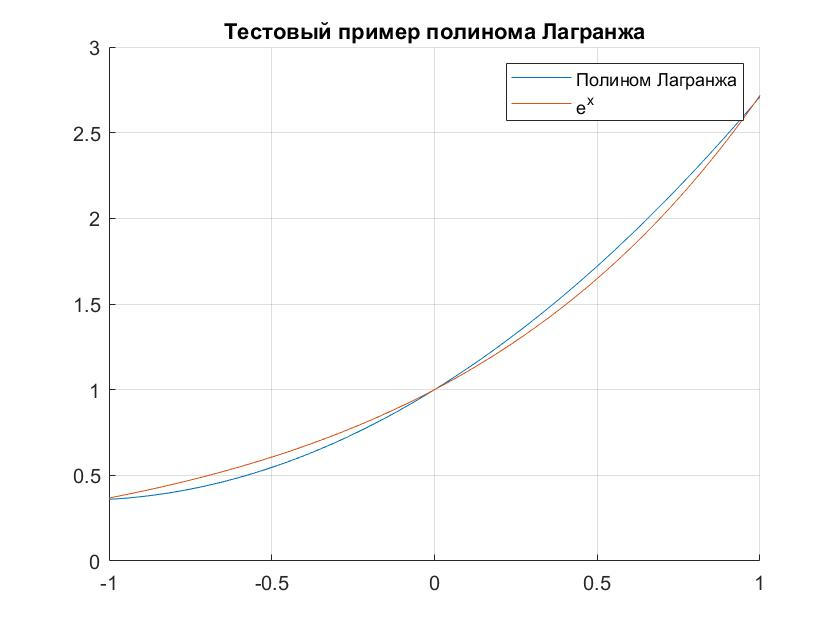
\includegraphics[width=0.7\linewidth]{test}
	\caption{Тестовый пример полинома Лагранжа}
	\label{fig:test}
\end{figure}
\section{Подготовка контрольных тестов}
Выполняется построение зависимости ошибки от количества узлов для равномерной и Чебышевской сетки для гладкой и разрывной функций.\\
Ошибка вводится следующим образом:
$$\epsilon = max|Ln(t) - f(t)|, t \in x^{h_1}$$
$$\lambda_{h_1} = \frac{\lambda_h}{100}$$
Помимо этого, выполнено построение графиков интерполяционного при разном количестве узлов: $n in {2, 4, 8, 10, 20}$\\
Графики см. в Приложении 1.\\

\section{Численный анализ}
Графики зависимости ошибки от количества узлов интерполяции для гладкой функции имеют следующий вид:\\ первоначально, при увеличении числа узлов интерполяции ошибка уменьшается. Затем ошибка начинает возрастать. Для чебышевской сетки рост ошибки начинается при большем количестве узлов.\\
Графики для разрывной функции имеют тот же вид.\\
Для гладкой функции ошибка
\end{document}
